% Benchmarks of SOD-ROM (Figure 1), TikZ version of python/rom/mkfig_c_systems.py.
% (a) shear frame; (b) cantilever, tip and mid-span loads; (c) with tip dashpot; (d) COST F3 beam, cubic tip spring;
% (e) two-well cantilever under base acceleration. Compile standalone, or \input the tikzpicture into the paper.
\documentclass[tikz,border=2pt]{standalone}
\usepackage{amsmath}
% scalars: A, E, I, L, P, \varOmega
\usetikzlibrary{arrows.meta,patterns,decorations.pathmorphing,calc}
\definecolor{mblue}{HTML}{0072BD}\definecolor{morange}{HTML}{D95319}
\definecolor{mgray}{HTML}{808080}\definecolor{mlgray}{HTML}{BFBFBF}\definecolor{mdred}{HTML}{A2142F}
\tikzset{
  beam/.style={mblue,line width=1.6pt},
  node dot/.style={circle,fill=mblue,inner sep=0pt,minimum size=3.2pt},
  load/.style={morange,-{Stealth[length=4pt]},line width=0.8pt},
  lbl/.style={font=\scriptsize},
  ground/.style={pattern=north east lines,draw=none},
  every node/.style={font=\footnotesize}}
% clamped wall at (#1); beam to the right
\newcommand{\clamp}[1]{%
  \fill[ground] ($(#1)+(-0.18,-0.55)$) rectangle ($(#1)+(0,0.55)$);
  \draw[line width=1pt] ($(#1)+(0,-0.55)$) -- ($(#1)+(0,0.55)$);
  %\foreach \yy in {-0.5,-0.3,...,0.5} \draw[line width=0.4pt] ($(#1)+(-0.18,\yy)$) -- ++(-0.12,-0.12);
  }
% hatched ground segment centred at (#1), half width #2
\newcommand{\groundline}[2]{%
  \fill[ground] ($(#1)+(-#2,-0.12)$) rectangle ($(#1)+(#2,0)$);
  \draw[line width=0.8pt] ($(#1)+(-#2,0)$) -- ($(#1)+(#2,0)$);}
% straight beam of length #2 cm with #3 elements, starting at (#1)
\newcommand{\fembeam}[3]{%
  \draw[beam] (#1) -- ++(#2,0);
  \foreach \k in {0,...,#3} \node[node dot] at ($(#1)+({#2*\k/#3},0)$) {};}
\begin{document}
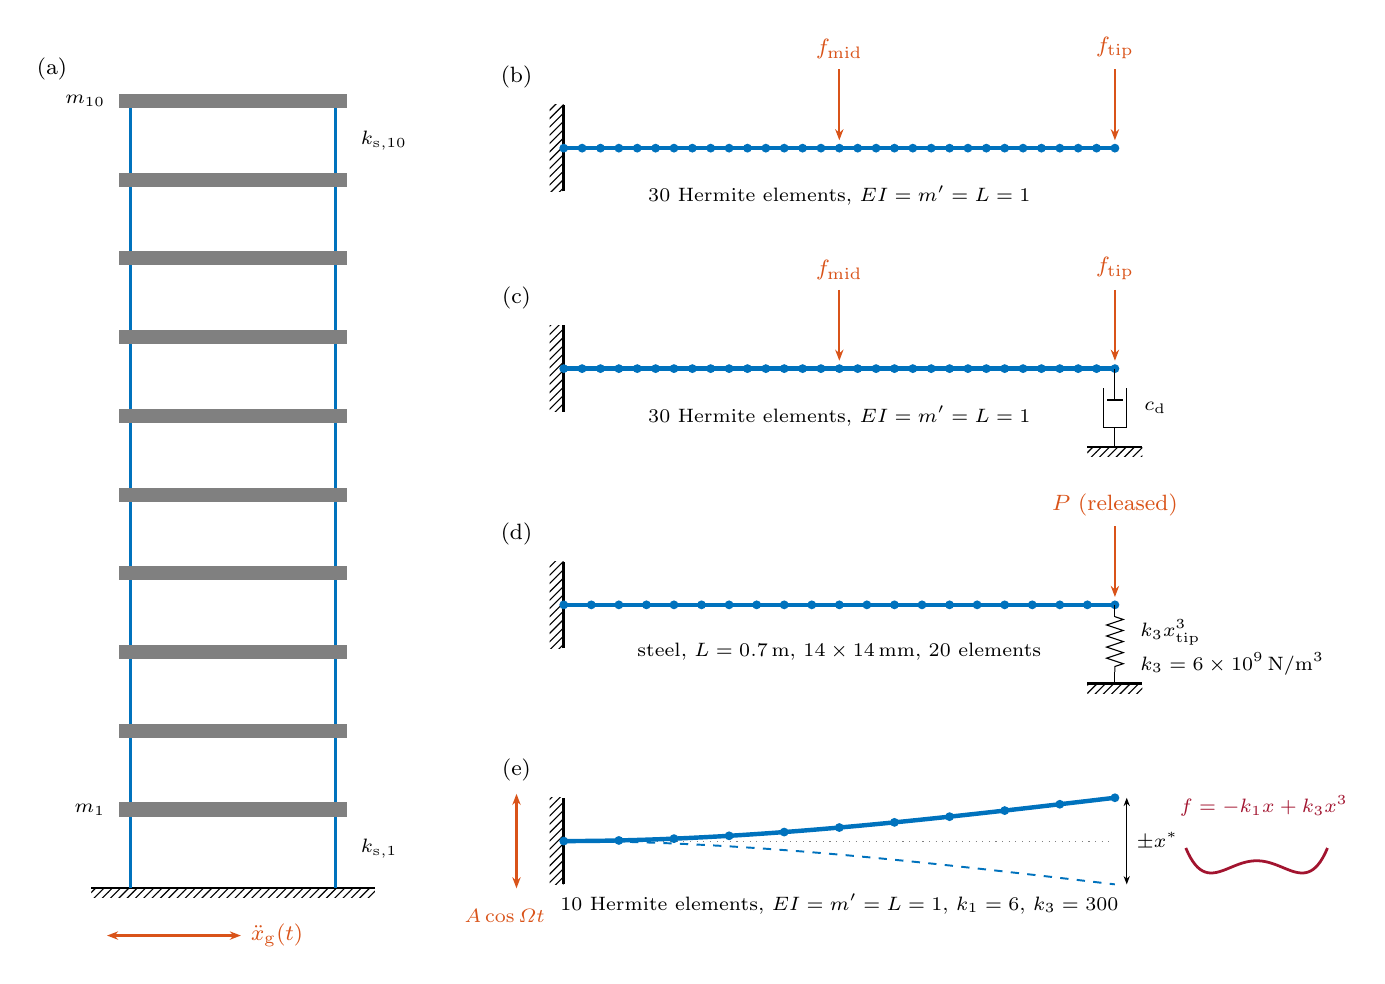
\begin{tikzpicture}
% ---------------- (a) shear frame ----------------
\begin{scope}[shift={(0,0)}]
  \def\H{1.0}\def\W{2.6}
  \groundline{\W/2,0}{1.8}
  \draw[mblue,line width=1.3pt] (0,0) -- (0,10*\H);
  \draw[mblue,line width=1.3pt] (\W,0) -- (\W,10*\H);
  \foreach \i in {1,...,10} \fill[mgray] (-0.15,{\i*\H-0.09}) rectangle (\W+0.15,{\i*\H+0.09});
  \node[lbl,left] at (-0.2,\H) {$m_1$};  \node[lbl,left] at (-0.2,10*\H) {$m_{10}$};
  \node[lbl,right] at (\W+0.2,0.5*\H) {$k_{\mathrm s,1}$}; \node[lbl,right] at (\W+0.2,9.5*\H) {$k_{\mathrm s,10}$};
  \draw[morange,{Stealth[length=4pt]}-{Stealth[length=4pt]},line width=0.8pt] (-0.3,-0.6) -- (1.4,-0.6)
    node[right,morange] {$\ddot x_{\mathrm g}(t)$};
  \node at (-1.0,10.4) {(a)};
\end{scope}
% ---------------- right column: beams, length 7 cm ----------------
\def\Lb{7}
% (b) cantilever with tip and mid-span loads
\begin{scope}[shift={(5.5,9.4)}]
  \clamp{0,0}\fembeam{0,0}{\Lb}{30}
  \draw[load] (\Lb/2,1.0) node[above,morange] {$f_{\mathrm{mid}}$} -- (\Lb/2,0.1);
  \draw[load] (\Lb,1.0) node[above,morange] {$f_{\mathrm{tip}}$} -- (\Lb,0.1);
  \node[lbl] at (\Lb/2,-0.6) {30 Hermite elements, $EI=m'=L=1$};
  \node at (-0.6,0.9) {(b)};
\end{scope}
% (c) with tip dashpot to ground
\begin{scope}[shift={(5.5,6.6)}]
  \clamp{0,0}\fembeam{0,0}{\Lb}{30}
  \draw[load] (\Lb/2,1.0) node[above,morange] {$f_{\mathrm{mid}}$} -- (\Lb/2,0.1);
  \draw[load] (\Lb,1.0) node[above,morange] {$f_{\mathrm{tip}}$} -- (\Lb,0.1);
  % dashpot
  \draw (\Lb,0) -- (\Lb,-0.4);
  \draw[thick] (\Lb-0.1,-0.4) -- (\Lb+0.1,-0.4);
  \draw (\Lb-0.15,-0.25) -- (\Lb-0.15,-0.75) -- (\Lb+0.15,-0.75) -- (\Lb+0.15,-0.25);
  \draw (\Lb,-0.75) -- (\Lb,-1.0); \groundline{\Lb,-1.0}{0.35}
  \node[lbl,right] at (\Lb+0.25,-0.5) {$c_{\mathrm d}$};
  \node[lbl] at (\Lb/2,-0.6) {30 Hermite elements, $EI=m'=L=1$};
  \node at (-0.6,0.9) {(c)};
\end{scope}
% (d) COST F3 beam, cubic spring from the tip to ground, released from a static tip load
\begin{scope}[shift={(5.5,3.6)}]
  \clamp{0,0}\fembeam{0,0}{\Lb}{20}
  \draw[load] (\Lb,1.0) node[above,morange] {$P$ (released)} -- (\Lb,0.1);
  \draw (\Lb,0) -- (\Lb,-0.15);
  \draw[decorate,decoration={zigzag,segment length=4pt,amplitude=3pt}] (\Lb,-0.15) -- (\Lb,-0.85);
  \draw (\Lb,-0.85) -- (\Lb,-1.0); \groundline{\Lb,-1.0}{0.35}
  \node[lbl,right] at (\Lb+0.2,-0.35) {$k_3x_{\mathrm{tip}}^3$};
  \node[lbl,right] at (\Lb+0.2,-0.75) {$k_3=6\times10^9$\,N/m$^3$};
  \node[lbl] at (\Lb/2,-0.6) {steel, $L=0.7$\,m, $14\times14$\,mm, 20 elements};
  \node at (-0.6,0.9) {(d)};
\end{scope}
% (e) two-well cantilever under harmonic base acceleration
\begin{scope}[shift={(5.5,0.6)}]
  \clamp{0,0}
  \draw[morange,{Stealth[length=4pt]}-{Stealth[length=4pt]},line width=0.8pt] (-0.6,-0.6) -- (-0.6,0.6);
  \node[lbl,morange] at (-0.75,-0.95) {$A\cos\varOmega t$};
  \draw[mgray,dotted] (0,0) -- (\Lb,0);
  % buckled shapes: static tip-load shape (3s^2 - s^3)/2, exaggerated to +-0.55 cm at the tip
  \draw[beam] plot[domain=0:1,samples=40] ({\Lb*\x},{0.55*(3*\x*\x-\x*\x*\x)/2});
  \foreach \k in {0,...,10} \node[node dot] at ({\Lb*\k/10},{0.55*(3*(\k/10)^2-(\k/10)^3)/2}) {};
  \draw[mblue,dashed,line width=0.7pt] plot[domain=0:1,samples=40] ({\Lb*\x},{-0.55*(3*\x*\x-\x*\x*\x)/2});
  \draw[{Stealth[length=3pt]}-{Stealth[length=3pt]},line width=0.4pt] (\Lb+0.15,0.55) -- (\Lb+0.15,-0.55);
  \node[lbl,right] at (\Lb+0.15,0) {$\pm x^*$};
  % double-well potential of the tip force
  \draw[mdred,line width=1pt] plot[domain=-1.8:1.8,samples=60] ({\Lb+1.8+0.5*\x},{-0.25+0.35*(-\x*\x/1.5+\x*\x*\x*\x/4)});
  \node[lbl,mdred,right] at (\Lb+0.7,0.45) {$f=-k_1x+k_3x^3$};
  \node[lbl] at (\Lb/2,-0.8) {10 Hermite elements, $EI=m'=L=1$, $k_1=6$, $k_3=300$};
  \node at (-0.6,0.9) {(e)};
\end{scope}
\end{tikzpicture}
\end{document}
